\part{固体物理}
\chapter{晶体结构与性质}
\section{常见晶体结构}
\subsection{凝聚态}
    \textbf{凝聚态}\index{凝聚态},指的是由大量粒子组成的、并且粒子间有很强的相互作用的系统,一般包括固体、液体以及介于二者之间的软物质(例如凝胶、液晶)。

    \textbf{固体}\index{固体}是凝聚态的一种特殊聚集形式。当压强与温度一定,且无外力作用时,固体的形状和体积保持不变——而液体则没有这种性质。固体由大量的原子(或离子)构成,每$1cm^3$体积中大约有$10^{23}$个粒子,大量粒子以一定的形式排列,我们将粒子排列的方式称为固体的结构。

    按照固体中粒子排列的有序度和对称性,固体可以分为晶体、非晶体和准晶体三类,如\autoref{fig:1-01}所示:
    \begin{itemize}[itemsep=0pt,parsep=0pt]
        \item \textbf{晶体}\index{晶体}:晶体中的组成粒子在空间周期性排列,称为长程序。
        \item \textbf{非晶体}\index{非晶体}:非晶体中的组成粒子在空间中不具备周期性,也并非完全无序,称为短程序。
        \item \textbf{准晶体}\index{准晶体}:准晶体介于晶体与非晶体之间。它的粒子分布是有序的,但不具备周期性,仅具备长程取向序。
    \end{itemize}
    具体来说,非晶体的排列是混乱无序的,或者说其规律仅适用于较小的空间内;而晶体与准晶体的排列则是有序规律的。然而,晶体可以无空隙地填充整个空间,准晶体同样可以填充空间,但不可避免的存在空隙。

    \begin{figure}[!htbp]
        \centering
        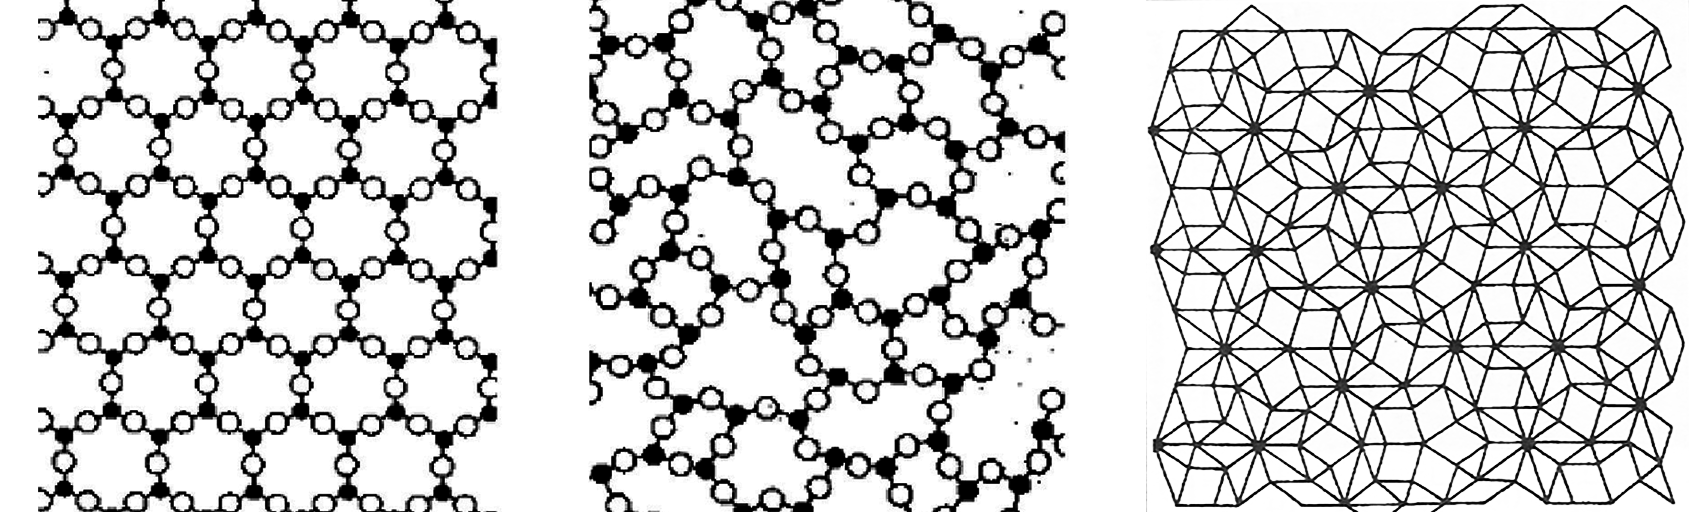
\includegraphics[width=\textwidth, keepaspectratio=true]{pic/1-01}
        \caption{晶体、非晶体与准晶体的粒子排列}
        \label{fig:1-01}
    \end{figure}

\subsection{晶格}
    晶体中,粒子排列的具体周期性结构称为\textbf{晶格}\index{晶格}。不同晶体具有不同的粒子排列结构,我们称为具有不同的晶格。
    
    我们在本节介绍若干种常见的晶体结构。为了便于理解,我们把晶格视为球体的堆积,即一个个原子呈球形,且彼此紧密的堆积在一起。

    \autoref{tab:1-1}引入下列晶格参数,从而方便地描述晶格特性:
    \begin{table}[!htbp]
        \centering
        \setlength{\tabcolsep}{1em}
        \begin{tabular}{lcl}
            \toprule
            晶格参数    &   字母表示    &   含义    \\
            \midrule
            晶格常数    &   $a$     &   标注某条棱的长度\\
            有效原子数  &           &   晶格内所含有的原子数\\
            配位数      &   $n$     &   与某原子距离最近的原子数\\
            最近邻距离  &           &   与某原子距离最近的原子的距离\\
            致密度      &   $\rho$  &   $\mbox{致密度}\rho=\frac{\mbox{有效原子数}\times \mbox{原子体积}}{\mbox{晶格体积}}$\\
            密排方向    &           &   在某个方向上原子密排\\
            \bottomrule
        \end{tabular}
        \caption{晶格常数}
        \label{tab:1-1}
    \end{table}

\newpage 
\subsubsection{第一类晶格:立方体结构}
    将同种粒子放在正方形的顶点上,即可得到平面的二维正方结构;\\
    同理我们推广到三维情况。所有的立方体结构晶格如\autoref{tab:1-2}所示。
    \begin{itemize}[itemsep=0pt,parsep=0pt]
        \item \textbf{简单立方}\index{简单立方}:将同种粒子放在立方体的顶点上,即为简单立方结构。\footnote{简单立方结构在自然界中极其罕见,目前唯一实例是钋($Po$)的$\alpha$相晶体}
        \item \textbf{面心立方}\index{面心立方}:在简单立方的基础上,若立方体面心还有一个粒子,即为面心立方结构。\footnote{应当指出,面心立方即为最密堆积的ABC结构。}
        \item \textbf{体心立方}\index{体心立方}:在简单立方的基础上,若立方体体心还有一个粒子,即为体心立方结构。
    \end{itemize}

    \begin{table}[!htbp]
        \centering
        \resizebox{\textwidth}{!}{
        \setlength{\tabcolsep}{1em}
        \begin{tabular}{ccccc}
                & 二维正方 & 简单立方 & 面心立方 & 体心立方\\
                & 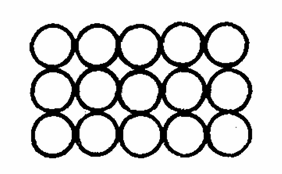
\includegraphics[height=6em, keepaspectratio=true]{pic/1-02} & 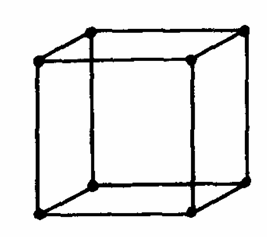
\includegraphics[height=6em, keepaspectratio=true]{pic/1-03} & 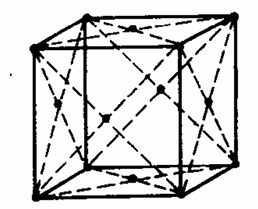
\includegraphics[height=6em, keepaspectratio=true]{pic/1-04} & 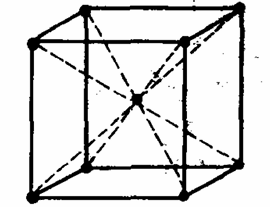
\includegraphics[height=6em, keepaspectratio=true]{pic/1-05}\\
            晶格常数$a$ & a & a & a & a \\
            密排方向    &沿边$a=2r$&沿棱$a=2r$&沿面对角线$\sqrt{2}a=4r$&沿体对角线$\sqrt{3}a=4r$\\
            有效原子数  &$4\times \frac{1}{4} = 1$&$8\times \frac{1}{8} = 1$&$8\times \frac{1}{8} + 6\times \frac{1}{2}= 4$&$8\times \frac{1}{8} + 1\times 1= 2$\\
            配位数$n$   &4&6&12&8\\
            最近邻距离  &$a$&$a$&$\frac{\sqrt{2}}{2}a$&$\frac{\sqrt{3}}{2}a$\\
            致密度$\rho$&&$\rho_1=\frac{1\times \frac{4}{3} \pi r^3}{(2r)^3} = \frac{\pi}{6}$&$\rho_2=\frac{4\times \frac{4}{3} \pi r^3}{(2\sqrt{2}r)^3} = \frac{\sqrt{2}}{6}\pi$&$\rho_3=\frac{2\times \frac{4}{3} \pi r^3}{(\frac{4}{\sqrt{3}}r)^3} = \frac{\sqrt{3}}{8}\pi$\\
        \end{tabular}
        }
        \caption{立方体结构晶格}
        \label{tab:1-2}
    \end{table}

\subsubsection{第二类晶格:密堆积结构}
    我们考虑这样的问题:如何排列,可以使得二维平面内可以放下最多的球体?这就是二维等径球最密堆积问题。可以证明,\autoref{fig:1-02}这样的排列是平面内的最密排列,称这种原子球在平面内最紧密排列的方式为\textbf{密排面}\index{密排面}。

    \begin{figure}[!htbp]
        \centering
        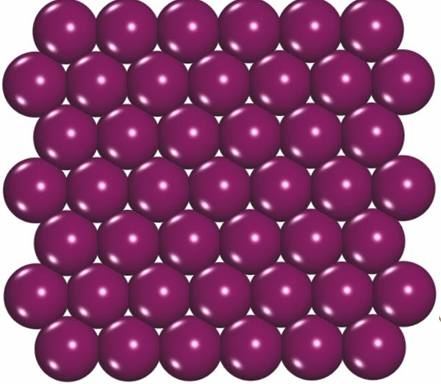
\includegraphics[height=8em, keepaspectratio=true]{pic/1-09}
        \caption{二维等径球最密堆积}
        \label{fig:1-02}
    \end{figure}

    仔细观察\autoref{fig:1-03}这样的密排面,我们应当注意到它具有两种不同的三角形空隙——一种三角形的尖尖朝上,如图中的第一排空隙B所示;另一种的三角形的尖尖朝下,如图中的第二排空隙C所示。两种空隙彼此交错。

    \begin{figure}[!htbp]
        \centering
        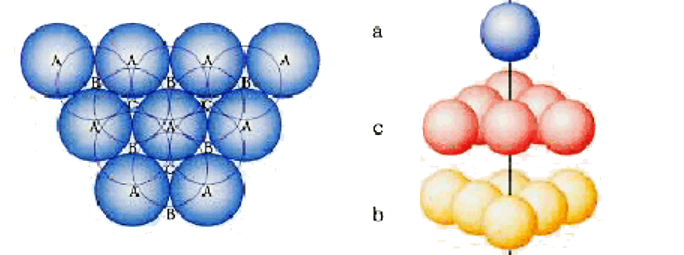
\includegraphics[height=8em, keepaspectratio=true]{pic/1-10}
        \caption{密排面的空隙}
        \label{fig:1-03}
    \end{figure}

    推广到三维情况,为了堆积得最紧密,由若干个这样的密排面一层层叠加起来,将一层的球心对准另一层的空隙。这就出现了两种堆叠方式,并由此形成了两种完全不同密堆积结构:AB型,与ABC型,如\autoref{fig:1-04}所示。
    
    顾名思义,第一种堆积方式即第一层的球心A对齐第二层的空隙B,并继续堆积第三层的球心A';第二种堆积方式则是第一层的球心先对齐第二层的空隙B,再对齐第三层的另一种空隙C,最后堆积新的一层的球心。
    
    \begin{figure}[!htbp]
        \centering
        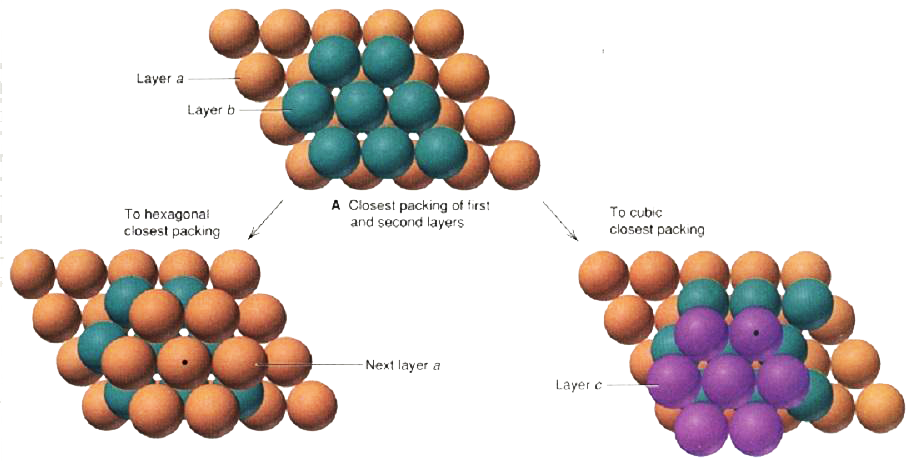
\includegraphics[height=12em, keepaspectratio=true]{pic/1-11}
        \caption{两种密堆积结构:AB型与ABC型}
        \label{fig:1-04}
    \end{figure}

    应当指出:ABC型堆积中,BC的顺序并不重要。根据观察的角度不同,空隙的指向也会变换,我们只要求BC两层空隙的角度相反。也可以认为,对于$\dots$\textcolor{red}{\textbf{ABC}}ABC$\dots$的堆积,我们从相反方向观察,就自然变成了$\dots$CB\textcolor{red}{\textbf{ACB}}A$\dots$的堆积。

    归纳密堆积结构晶格如\autoref{tab:1-3}所示:
    \begin{table}[!htbp]
        \centering
        \resizebox{\textwidth}{!}{
        \setlength{\tabcolsep}{1em}
        \begin{tabular}{cccc}
                & 二维六角 & 六角密排AB & 面心立方ABC\\
                & 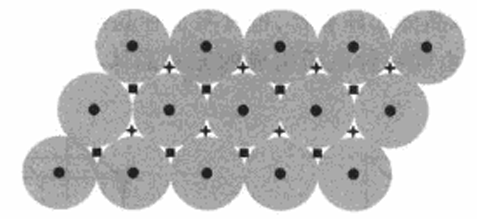
\includegraphics[height=4em, keepaspectratio=true]{pic/1-06} & 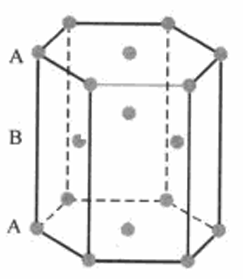
\includegraphics[height=8em, keepaspectratio=true]{pic/1-07} & 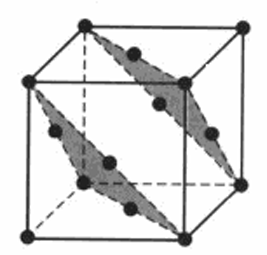
\includegraphics[height=8em, keepaspectratio=true]{pic/1-08}\\
            晶格常数$a$ & a & a \& c & a \\
            密排方向    &沿两近邻粒子方向$a=2r$&水平方向$a=2r$垂直方向$h=\frac{\sqrt{6}}{2}a=\frac{c}{2}$&沿面对角线$\sqrt{2}a=4r$\\
            有效原子数  &1&2&4\\
            配位数$n$   &6&12&12\\
            最近邻距离$a$&$a$&$a$&$\frac{\sqrt{2}}{2}a$\\
            致密度$\rho$&&$\rho_1=\frac{2\times \frac{4}{3} \pi r^3}{(\frac{\sqrt{3}}{4}a)^3 \times 2\times h} = \frac{\sqrt{2}}{6} \pi$&$\rho_2=\frac{4\times \frac{4}{3} \pi r^3}{(2\sqrt{2}r)^3} = \frac{\sqrt{2}}{6}\pi$\\
        \end{tabular}
        }
        \caption{密堆积结构晶格}
        \label{tab:1-3}
    \end{table}

    我们给出这样的两个要点:
    \begin{enumerate}[itemsep=0pt,parsep=0pt]
        \item \textbf{面心立方}既可以从立方体结构的角度考虑,而如果我们从立方体的体对角线看过去——这就是密堆积结构的ABC型。
        \item \textbf{面心立方}与\textbf{体心立方}互为倒格子。这将是\autoref{chap:2}的重要结论。
    \end{enumerate}

\subsubsection{第三类晶格:复式晶格}
    上述的第一类晶格与第二类晶格,常见于同一种原子所组成的单质晶体。我们现在介绍一些由多种原子或离子所组成的化合物晶体的晶格。

    我们介绍简单晶格与复式晶格的概念。化合物常表现为复式晶格。
    \begin{itemize}[itemsep=0pt,parsep=0pt]
        \item \textbf{简单晶格}\index{简单晶格}:所有原子完全等价。将晶格从一个原子向另一个原子作平移后,新得到的晶格与原晶格完全复原。
        \item \textbf{复式晶格}\index{复式晶格}:含有两种及以上不等价的所有原子或离子。将晶格从一个粒子向另一个粒子作平移后,无法复原晶格。复式晶格总可以看成若干种简单晶格的套构。
    \end{itemize}

    我们以下面三种化合物晶体为例,研究复式晶格及其套构。

    \textbf{CsCl结构}\index{CsCl结构}:CsCl结构与体心立方类似,但位于体心与位于顶点的分别是两种不同的离子,每种离子位于8个异类离子构成的立方体的中心。如果考虑整个晶格,“顶点”与“体心”的概念是相对的,二者完全等效。

    \textbf{NaCl结构}\index{NaCl结构}:将$Na^+$离子和$Cl^-$离子交替放在一个简单立方晶格上,构成NaCl结构。显然$Na^+$离子与$Cl^-$离子两类粒子不等价。实际上所有的碱金属-卤化物晶体都具有NaCl结构。

    \textbf{ZnS结构}\index{金刚石结构}:闪锌矿ZnS的结构与面心立方类似,由面心立方的中心到各个顶角作8条对角线,并在其中4条互不相邻的对角线的中点放置另一种粒子。两种粒子位置不等价,每种粒子处于4个最近邻异类粒子所构成的四面体的中心。两种粒子各自构成的四面体在取向上相差$90^{\circ}$。金刚石与半导体材料锗、硅也具有该结构。

    归纳复式晶格如\autoref{tab:1-4}所示:
    \begin{table}[!htbp]
        \centering
        \resizebox{\textwidth}{!}{
        \setlength{\tabcolsep}{1em}
        \begin{tabular}{cccc}
                & CsCl结构 & NaCl结构 & 金刚石结构\\
                & 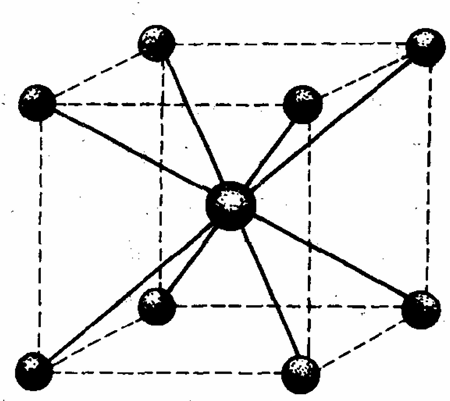
\includegraphics[height=8em, keepaspectratio=true]{pic/1-12} & 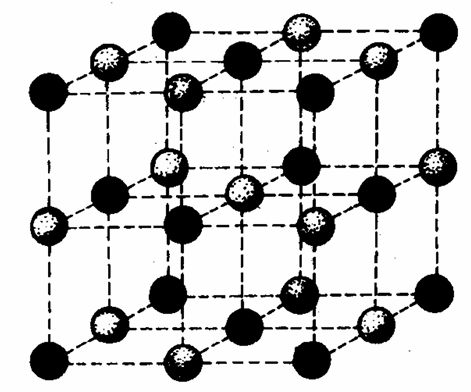
\includegraphics[height=8em, keepaspectratio=true]{pic/1-13} & 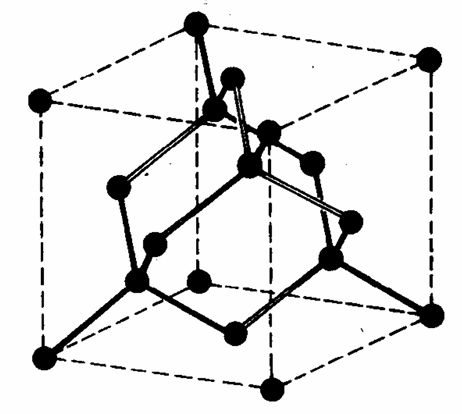
\includegraphics[height=8em, keepaspectratio=true]{pic/1-14}\\
            有效原子数  &2&8&8\\
            配位数$n$   &8&6&4\\
            套构情况    &简单立方沿对角线方向$\frac{1}{2}$套构&面心立方沿棱方向$\frac{1}{2}$套构&体心立方沿对角线方向$\frac{1}{4}$套构\\
        \end{tabular}
        }
        \caption{复式晶格}
        \label{tab:1-4}
    \end{table}
    
\section{晶体的周期性}\index{晶体的周期性}
    凡是晶体就具有\textbf{周期性},也称为平移对称性。我们可以用一个最小的、完全等价的结构单元,在空间无限重复,从而得到整个晶格。这个能够充分反映晶体结构特征的全同结构单元称为\textbf{晶胞}\index{晶胞}或\textbf{基元}。晶胞有多种选取方式,最实用的是单胞与原胞两种。

    为了研究晶体的周期性即平移对称性,我们忽略晶体中的具体粒子,将不等价的粒子(即基元)抽象为几何点,从而原本复杂的晶格被抽象为纯粹的几何点阵。这样的点阵称为\textbf{布拉菲点阵}或\textbf{布拉菲格子}\index{布拉菲格子}。

\subsection{布拉菲点阵}
    布拉菲点阵作为数学概念,是由分立点所构成的无限阵列,从阵列的任何一个结点去看,周围各结点的分布与方位都是精确相同的。

    对于晶格来说,我们通过将基元抽象为几何点得到布拉菲格子。于是我们有:
    \[
        \mbox{<晶体>}=\mbox{<基元>}+\mbox{<布拉菲点阵>}
    \]
    
    我们考虑二维平面与三维空间中有多少种布拉菲格子,即几何点在二维平面(三维空间)有多少种周期性的规律排布。

\subsubsection{二维布拉菲格子}
    共存在5种二维布拉菲格子,又可分为4种晶系。我们记二维点阵的两边为$a$、$b$,第三边为$c$;夹角为$\gamma$,其分类标准及转化关系如\autoref{tab:1-5}所示:

    \begin{table}[!htbp]
        \centering
        \resizebox{\textwidth}{!}{
        \setlength{\tabcolsep}{1em}
        \begin{tabular}{ccccc}
            \toprule
            布拉菲格子& 边长特征        & 夹角特征                   & 晶系     & 转化关系 \\
            \midrule
            斜方      & $a\neq b$      & $\gamma \neq 90^{\circ}$  & 斜方晶系 & \multirow{5}{*}[-0.5em]{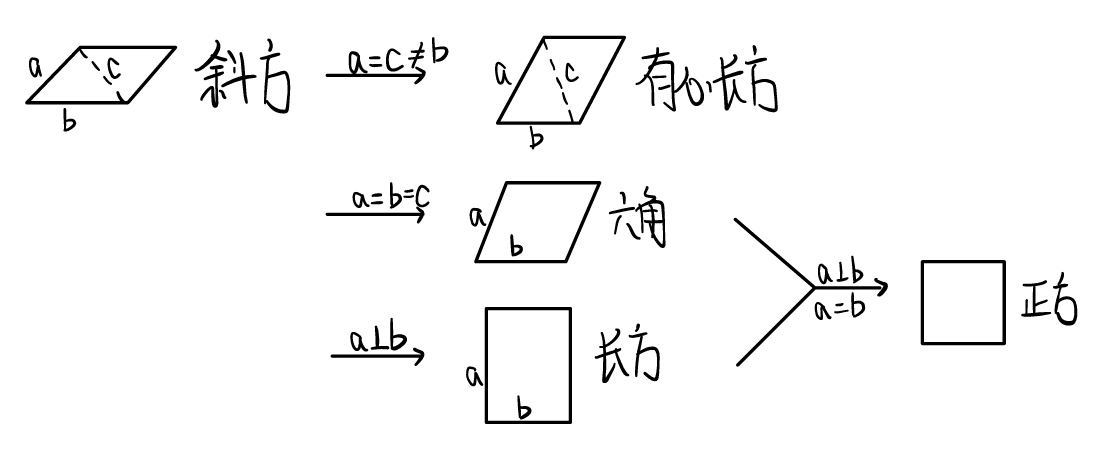
\includegraphics[height=7em, keepaspectratio=true]{pic/1-16}}\\
            有心长方  & $a = c \neq b$ & $\gamma \neq 90^{\circ}$  & \multirow{2}{*}{长方晶系} &\\
            长方      & $a\neq b$      & $\gamma=90^{\circ}$       &         &  \\
            六角      & $a=b$          & $\gamma=60^{\circ}$       & 六角晶系 &  \\
            正方      & $a=b$          & $\gamma=90^{\circ}$       & 正方晶系 &  \\
            \bottomrule
        \end{tabular}
        }
        \caption{二维布拉菲格子}
        \label{tab:1-5}
    \end{table}

    \autoref{fig:1-05}可以证明,左侧的所谓“有心正方”晶格实际上等价于“正方”,即5种二维布拉菲格子已经完备。

    \begin{figure}[!htbp]
        \centering
        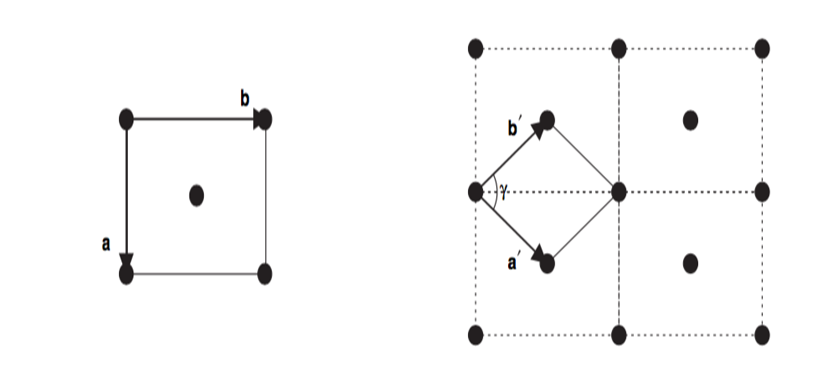
\includegraphics[height=9em, keepaspectratio=true]{pic/1-17}
        \caption{不存在“有心正方”晶格}
        \label{fig:1-05}
    \end{figure}

\subsubsection{三维布拉菲格子}
    共存在14种二维布拉菲格子,又可分为7种晶系。我们记三维点阵的三边为$a$、$b$、$c$,三个方向的夹角为$\alpha$、$\beta$、$\gamma$。如\autoref{tab:1-6}所示:

    \begin{table}[!htbp]
        \centering
        \resizebox{\textwidth}{!}{
        \setlength{\tabcolsep}{1em}
        \begin{tabular}{ccccc}
            \toprule
            晶系     & 边长特征         & 夹角特征                   & 布拉菲格子  & 示意图 \\
            \midrule
            三斜晶系 & $a\neq b\neq c$ & $\alpha \neq \beta \neq \gamma$                 & 简单三斜    & \multirow{7}{*}[-1.5em]{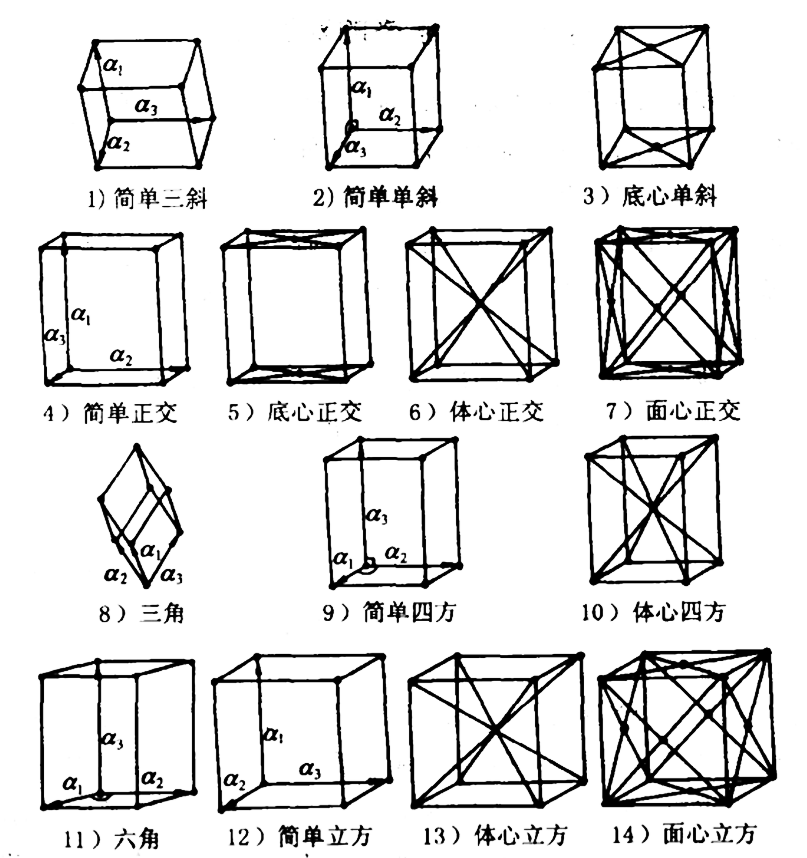
\includegraphics[height=10em, keepaspectratio=true]{pic/1-18}} \\
            单斜晶系 & $a\neq b\neq c$ & $\alpha=\gamma=90^{\circ}\neq \beta $           & 简单单斜、底心单斜    & \\
            三角晶系 & $a=b=c$         & $\alpha=\beta=\gamma\neq90^{\circ}<120^{\circ}$ & 三角    & \\
            正交晶系 & $a\neq b\neq c$ & $\alpha=\beta=\gamma=90^{\circ}$                & \makecell{简单正交、底心正交、\\体心正交、面心正交}    & \\
            四角晶系 & $a=b\neq c$     & $\alpha=\beta=\gamma=90^{\circ}$                & 简单四角、体心四角    & \\
            六角晶系 & $a=b\neq c$     & $\alpha=\beta=90^{\circ}, \gamma=120^{\circ}$   & 六角    & \\
            正方晶系 & $a=b=c$         & $\alpha=\beta=\gamma=90^{\circ}$                & \makecell{简单立方、体心立方、\\面心立方}    & \\
            \bottomrule
        \end{tabular}
        }
        \caption{三维布拉菲格子}
        \label{tab:1-6}
    \end{table}

    与二维平面不存在所谓“有心正方”同理,三维空间不存在所谓“底心立方”、“面心正方”、“体心单斜”晶格,实际上等价于“简单立方”、“体心正方”、“底心单斜”,证明如\autoref{fig:1-06}所示。这也说明了14种三维布拉菲格子的完备性。

    \begin{figure}[!htbp]
        \centering
        \begin{minipage}[t]{0.3\linewidth}
            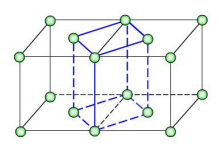
\includegraphics[width=1\linewidth, keepaspectratio=true]{pic/1-19}
            \subcaption{“底心立方”}
        \end{minipage}
        \hfill
        \begin{minipage}[t]{0.3\linewidth}
            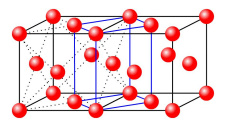
\includegraphics[width=1\linewidth, keepaspectratio=true]{pic/1-20}
            \subcaption{“面心正方”}
        \end{minipage}
        \hfill
        \begin{minipage}[t]{0.3\linewidth}
            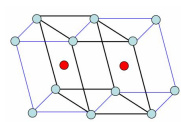
\includegraphics[width=1\linewidth, keepaspectratio=true]{pic/1-21}
            \subcaption{“体心单斜”}
        \end{minipage}
        \caption{不存在“底心立方”、“面心正方”、“体心单斜”晶格}
        \label{fig:1-06}
    \end{figure}

    布拉菲点阵是晶格的数学抽象。只要将基元按照布拉菲点阵排布,就可以还原晶体结构。同一种布拉菲点阵可以对应不同的晶体结构,但其平移对称性是一致的。

\subsection{单胞和原胞}
    三维晶格的晶胞通常是一个平行六面体,沿着某点出发的三条边取单位矢量$\vec{a_1}$、$\vec{a_2}$、$\vec{a_3}$,即晶胞的单位边矢量,这就是\textbf{晶格基矢}\index{晶格基矢}。晶胞所占的体积$\Omega=(\vec{a_1}\cdot \vec{a_2})\times \vec{a_3}$。

    现在研究晶胞的选取,常选取单胞或原胞作为晶胞:
    \begin{itemize}[itemsep=0pt,parsep=0pt]
        \item \textbf{单胞}\index{单胞}:反映晶格的宏观对称特性,常选取立方晶胞,其三条基矢沿着晶体的结晶轴方向,且尽可能构成正交系。
        \item \textbf{原胞}\index{原胞}:指晶格体积最小的周期性单元,可通过任意两结点的平移矢量$\vec{R}$不重不漏密排整个空间。原胞中只含有一个结点。原胞的三条基矢沿原胞的边的方向。
    \end{itemize}

    实际上单胞与原胞有多种取法。在晶体学中对各种晶格的单胞与原胞的选取做了规定,\autoref{tab:1-7}归纳了常用晶体所选取的单胞与原胞:
    \begin{table}[!htbp]
        \centering
        \resizebox{\textwidth}{!}{
        \setlength{\tabcolsep}{1em}
        \begin{tabular}{cclcl}
            \toprule
            晶格类型 & \multicolumn{2}{c}{单胞} & \multicolumn{2}{c}{原胞}\\
            \midrule
            简单立方 & 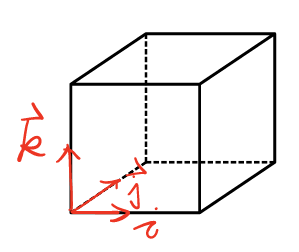
\includegraphics[valign=m, height=4em, keepaspectratio=true]{pic/1-22} & $
            \begin{cases}
            \vec{a_1}=a\vec{i}\\
            \vec{a_2}=a\vec{j}\\
            \vec{a_3}=a\vec{k}\\
            \end{cases}
            $ & 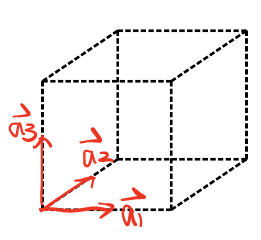
\includegraphics[valign=m, height=4em, keepaspectratio=true]{pic/1-24} & $
            \begin{cases}
            \vec{a_1}=a\vec{i}\\
            \vec{a_2}=a\vec{j}\\
            \vec{a_3}=a\vec{k}\\
            \end{cases}
            $ \\
            面心立方 & 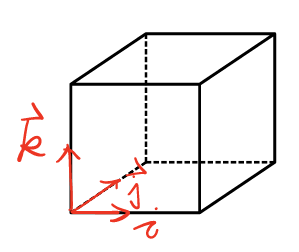
\includegraphics[valign=m, height=4em, keepaspectratio=true]{pic/1-22} & $
            \begin{cases}
            \vec{a_1}=a\vec{i}\\
            \vec{a_2}=a\vec{j}\\
            \vec{a_3}=a\vec{k}\\
            \end{cases}
            $ & 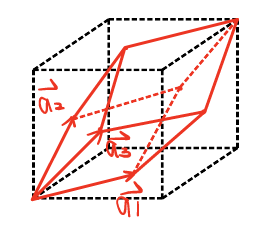
\includegraphics[valign=m, height=4em, keepaspectratio=true]{pic/1-25} & $
            \begin{cases}
            \vec{a_1}=\frac{a}{2}(\vec{i}+\vec{j})\\
            \vec{a_2}=\frac{a}{2}(\vec{j}+\vec{k})\\
            \vec{a_3}=\frac{a}{2}(\vec{k}+\vec{i})\\
            \end{cases}
            $ \\
            体心立方 & 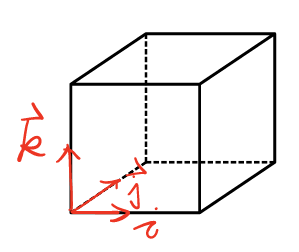
\includegraphics[valign=m, height=4em, keepaspectratio=true]{pic/1-22} & $
            \begin{cases}
            \vec{a_1}=a\vec{i}\\
            \vec{a_2}=a\vec{j}\\
            \vec{a_3}=a\vec{k}\\
            \end{cases}
            $ & 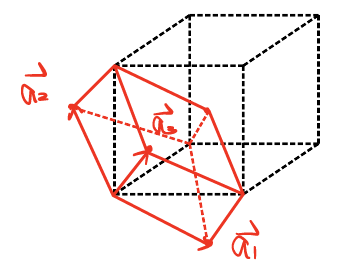
\includegraphics[valign=m, height=4em, keepaspectratio=true]{pic/1-26} & $
            \begin{cases}
            \vec{a_1}=\frac{a}{2}(\vec{i}+\vec{j}-\vec{k})\\
            \vec{a_2}=\frac{a}{2}(\vec{j}+\vec{k}-\vec{i})\\
            \vec{a_3}=\frac{a}{2}(\vec{k}+\vec{i}-\vec{j})\\
            \end{cases}
            $ \\
            六角密排 & 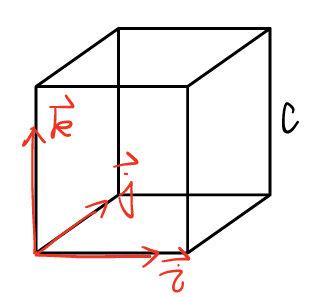
\includegraphics[valign=m, height=4em, keepaspectratio=true]{pic/1-23} & $
            \begin{cases}
            \vec{a_1}=a\vec{i}\\
            \vec{a_2}=a\vec{j}\\
            \vec{a_3}=c\vec{k}\\
            \end{cases}
            $ & 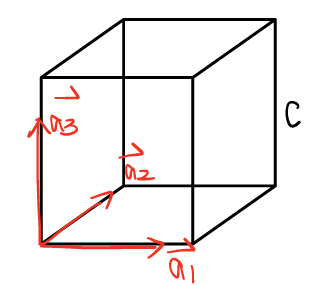
\includegraphics[valign=m, height=4em, keepaspectratio=true]{pic/1-27} & $
            \begin{cases}
            \vec{a_1}=a\vec{i}\\
            \vec{a_2}=\frac{a}{2}\vec{i}+\frac{\sqrt{3}a}{2}\vec{j}\\
            \vec{a_3}=c\vec{k}\\
            \end{cases}
            $ \\
            \bottomrule
        \end{tabular}
        }
        \caption{单胞与原胞的选取}
        \label{tab:1-7}
    \end{table}

    观察发现:单胞实际上是扩大了的原胞,是较大的周期单元;某些情况单胞与原胞相同。

\subsection{晶体的平移对称性}
\subsubsection{点阵的残缺的平移不变性}
    对于二维基矢$\{\vec{a_1}, \vec{a_2}\}$或三维基矢$\{\vec{a_1}, \vec{a_2}\, \vec{a_3}\}$,点阵中的自原点到每个结点的位置矢量$\vec{R_l}$可以写成
    \[
        \vec{R_l}=l_1\vec{a_1}+l_2\vec{a_2}+l_3\vec{a_3}
    \]
    其中$\{l_1, l_2, l_3\}$取任意整数时,位置矢量$\vec{R_l}$所指向的端点的集合将包含且仅包含整个点阵全部的结点。

    由此可知,点阵并不对任意的平移不变,而只对一组离散的平移矢量$\vec{R_l}$(其中$l_1, l_2, l_3\in \mathbb{N}$)具有不变性,称为残缺的平移不变性。

    此时,点阵中的任意结点由$l_1, l_2, l_3$的组合$(l_1, l_2, l_3)$唯一确定,布拉菲格子则是所有点$(l_1, l_2, l_3)$的集合。

\subsubsection{晶体物理性质的周期性}
    我们知道:
    \[
        \mbox{<晶体>}=\mbox{<基元>}+\mbox{<布拉菲点阵>}
    \]
    
    对于某个晶胞基元,其中第$\alpha$个粒子相对于晶胞原点有相对位移$\vec{r_\alpha}$。实际的晶格可以看成:在布拉菲点阵的每个结点上放置一个晶胞基元,晶胞基元中的粒子与结点间的相对位移即为$\vec{r_\alpha}$。只要将晶胞基元按照布拉菲格子排布,就能得到晶体的结构。

    则此时晶格中任意粒子的位置矢量可以写为:
    \[
        \vec{R_l}=\vec{r_\alpha}+l_1\vec{a_1}+l_2\vec{a_2}+l_3\vec{a_3}
        \quad (\alpha = 1,2,\dots)
    \]

    如果晶体中所有晶胞基元都严格处在布拉菲格子所确定的结点上,那么晶体内的一切物理量$V(\vec{r})$,都精确的是$\vec{R_l}$的周期函数,即:
    \[
        V(\vec{r})=V(\vec{r}+\vec{R_l})
    \]
    其中$\vec{r}$是坐标原点到任意位置的位移矢量。

\section{晶体的方向性}\index{晶体的方向性}
    晶体的一个基本特点是具有\textbf{方向性},沿晶格的不同方向晶体性质不同。这种性质差异被称为\textbf{各向异性}\index{各向异性}。这是因为单晶材料内部原子排列具有方向性,不同晶面方向上,原子的排列密度、原子间的结合强度、电子的运动方式等等都会有所不同,从而导致性质上的差异。

    我们在本节关注如何区别和描述晶格中的方向。
\subsection{晶向}
\subsubsection{晶列}
    在布拉菲点阵中,过原点和任意的一个结点可以确定一条直线。由于结点呈周期性排列,用一族这样平行且等间距的直线可以将整个点阵包括无遗,如\autoref{fig:1-07}中的虚线或实线所示。这样的一族直线我们称为\textbf{晶列}\index{晶列}。

    \begin{figure}[!htbp]
        \centering
        \begin{minipage}[t]{0.45\linewidth}
            \centering    
            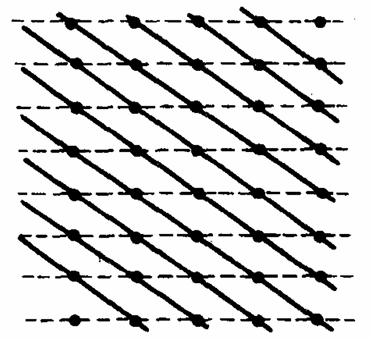
\includegraphics[height=8em, keepaspectratio=true]{pic/1-28}
            \caption{晶列}
            \label{fig:1-07}
        \end{minipage}
        \hfill
        \begin{minipage}[t]{0.45\linewidth}
            \centering
            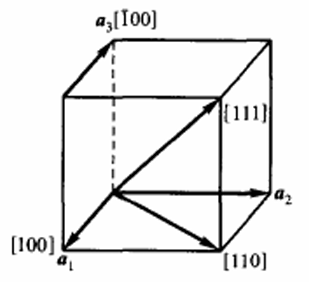
\includegraphics[height=8em, keepaspectratio=true]{pic/1-29}
            \caption{简单立方晶格的晶向}
            \label{fig:1-08}
        \end{minipage}
    \end{figure}
    
    由于布拉菲点阵中有无限个结点,也就有无限多条方向彼此不同的直线族,从而点阵中有无限族晶列。每一族晶列确定了一个方向,即\textbf{晶向}\index{晶向}。如果从一个结点沿着某晶列方向到最近邻结点的平移矢量为:
    \[
        \vec{R_l}=l_1\vec{a_1}+l_2\vec{a_2}+l_3\vec{a_3}
    \]
    则用$l_1$、$l_2$、$l_3$标志该晶列所对应的晶向,记为$[l_1, l_2, l_3]$,称为\textbf{晶向指数}\index{晶向指数}。由于平移矢量$\vec{R_l}$是最近邻原子间的位移,$l_1$、$l_2$、$l_3$一定是互质的整数,按照惯例若$l_1$、$l_2$、$l_3$为负数,则上标一横,如$-l_i$记为$\overline{l_i}$。

    以简单立方晶格中的晶向为例,如\autoref{fig:1-08}所示,其边、面对角线、体对角线的晶向指数依次为$[100]$、$[110]$、$[111]$。

\subsubsection{等效晶向}
    由于晶格具有对称性,某些晶向上晶格结构和晶学性质是相同的,我们称这些晶向是等效的,即\textbf{等效晶向}\index{等效晶向}。

    例如,立方晶格的边一共有$[100]$、$[\overline{1}00]$、$[010]$、$[0\overline{1}0]$、$[001]$、$[00\overline{1}]$六个晶向,考虑晶格的平移对称性,晶体在这些方向上的性质是完全相同的。我们用$<l_1,l_2,l_3>$来标志一组对称且等效的晶向,即$<100>$。

    边晶向、面对角线晶向、体对角线晶向总结如\autoref{tab:1-8}所示:
    \begin{table}[!htbp]
        \centering
        \resizebox{\textwidth}{!}{
        \setlength{\tabcolsep}{1em}
        \begin{tabular}{cccc}
                   & 边       & 面对角线 & 体对角线  \\
                   & 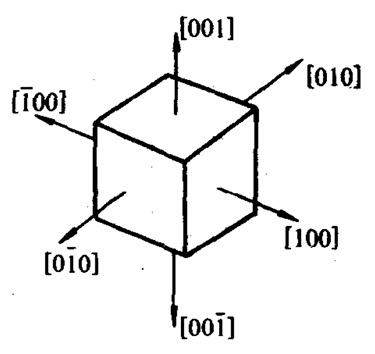
\includegraphics[height=8em, keepaspectratio=true]{pic/1-30} & 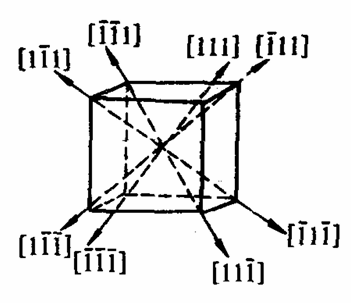
\includegraphics[height=8em, keepaspectratio=true]{pic/1-31} & 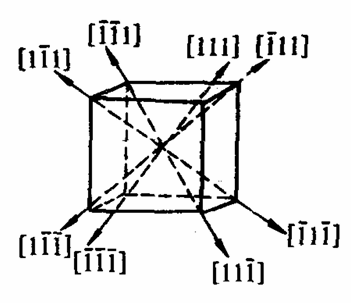
\includegraphics[height=8em, keepaspectratio=true]{pic/1-32} \\
            数目    & 6       &     12  &     8    \\
            等效晶向& $<100>$ & $<110>$ & $<111>$ \\
        \end{tabular}
        }
        \caption{等效晶向}
        \label{tab:1-8}
    \end{table}

    \textcolor{red}{一般晶向用$[l_1, l_2, l_3]$标志,系列晶向用$<l_1,l_2,l_3>$标志}

\subsection{晶面}
\subsubsection{晶面}
    在布拉菲点阵中,由于结点呈周期性排列,用一族平行且等间距的平面可以将整个点阵包括无遗,如\autoref{fig:1-09}所示。这样的一族平面我们称为\textbf{晶面}\index{晶面}。

    \begin{figure}[!htbp]
        \centering    
        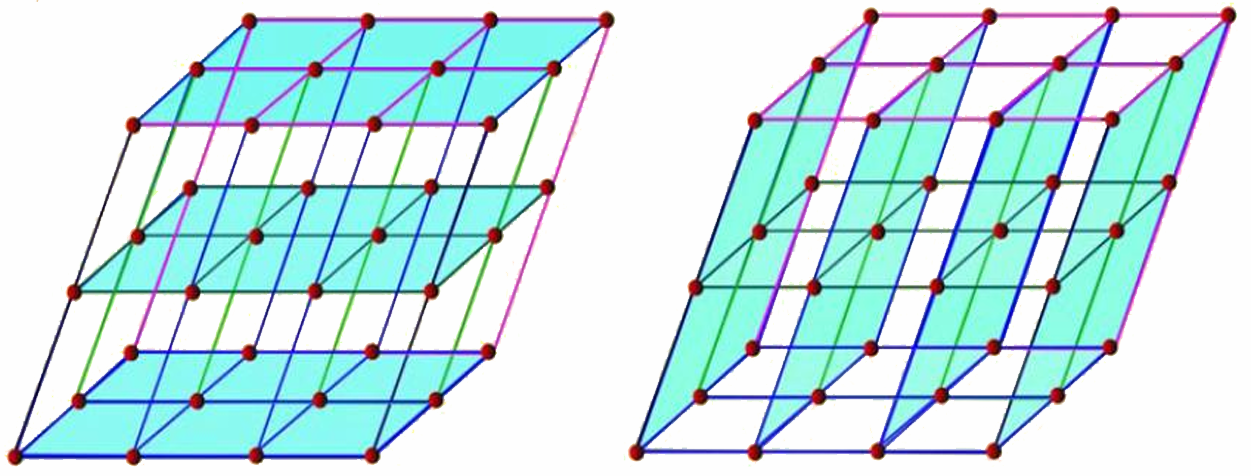
\includegraphics[height=7em, keepaspectratio=true]{pic/1-33}
        \caption{晶面}
        \label{fig:1-09}
    \end{figure}

    由于布拉菲点阵中有无限个结点,也就有无限多个方向彼此不同的平面族,从而点阵中有无限族晶面。每一族晶面确定了一个方向,即该族平面的法线方向。在数学上,我们可以用该平面法线的方向余弦,或者该平面在坐标轴上的截距来描述一个平面的方向——我们接下来将看到,这两种表示实际上是等价的。

    对于晶格中的一组平行且等距的晶面,将完全无遗地包括所有结点选取某个结点作为原点,以晶胞基矢为坐标轴建立坐标系,如\autoref{fig:1-10}所示。
    
    记晶面的法线方向为$\vec{e_n}$,晶面间距为$d$。指向第$\mu$个晶面($\mu$为整数)任意位置的位矢为$\vec{X}$,该晶面在坐标轴上的截距依次为$r_\mu a$、$s_\mu a$、$t_\mu a$。

    \begin{figure}[!htbp]
        \centering    
        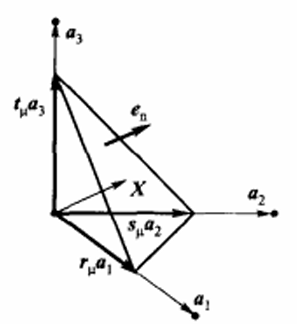
\includegraphics[height=8em, keepaspectratio=true]{pic/1-34}
        \caption{晶面的方向余弦}
        \label{fig:1-10}
    \end{figure}

    则有
    \[
        \vec{X} \cdot \vec{e_n} = \mu d
    \]
    
    将该晶面与坐标轴的交点代入可得:
    \[
    \begin{cases}
        r_\mu \vec{a_1} \cdot \vec{e_n} = r_\mu \cos (\vec{a_1}, \vec{e_n}) = \mu d \\
        s_\mu \vec{a_2} \cdot \vec{e_n} = s_\mu \cos (\vec{a_2}, \vec{e_n}) = \mu d \\
        t_\mu \vec{a_1} \cdot \vec{e_n} = t_\mu \cos (\vec{a_3}, \vec{e_n}) = \mu d \\
    \end{cases}
    \]

    联立可得:
    \[
        \cos (\vec{a_1}, \vec{e_n}) : \cos (\vec{a_1}, \vec{e_n}) : \cos (\vec{a_1}, \vec{e_n}) = \frac{1}{r_\mu} : \frac{1}{r_\mu} : \frac{1}{r_\mu}
    \]

    即:晶面法线方向的方向余弦之比,等于晶面与对应方向坐标轴截距的倒数之比。因此方向余弦和截距表述晶面方向是等价的,常用晶面与坐标轴的截距来表示晶面方向。

    进一步证明该组截距均为有理数。考察单位基矢处的结点,即$(1,0,0)$、$(0,1,0)$、$(0,0,1)$三个结点,由于晶面完全无遗包括所有结点,必然存在若干晶面经过该三个结点。不失一般的,我们记第$\mu_1$、$\mu_2$、$\mu_3$个晶面经过这三个结点。某些情况下可能存在一个晶面同时经过多个结点,此时相应地调整$\mu_1=\mu_2$即可。

    于是,第$\mu_i$个晶面在$\vec{a_i}$坐标轴上的截距为单位1,从而第$\mu$个晶面在坐标轴上的截距有:
    \[
        r_\mu = \frac{\mu}{\mu_1}, \\
        s_\mu = \frac{\mu}{\mu_2}, \\
        t_\mu = \frac{\mu}{\mu_3}
    \]
    其中$\mu$、$\mu_1$、$\mu_2$、$\mu_3$均为整数。
    
    则$r_\mu a$、$s_\mu a$、$t_\mu a$均是两个整数之比,必为有理数。

\subsubsection{晶面指数}
    若第一个晶面在坐标轴上的截距为$r_1 a$、$s_1 a$、$t_1 a$,取截距的倒数$h_1 = \frac{1}{r_1 a}, h_2 = \frac{1}{s_1 a}, h_3 = \frac{1}{t_1 a}$来标志该族晶面。若晶面在坐标轴上无截距,即截距无穷大,规定倒数为0。定义$(h_1, h_2, h_3)$为晶面指数,用来反映晶面所确定的方向。一般要求$h_1, h_2, h_3$互质。

    确定晶面指数的程序可以归纳为:
    \begin{enumerate}[itemsep=0pt,parsep=0pt]
        \item \textbf{找截距}:在一组晶面中,找出任一晶面在基矢坐标轴上的截距$r$、$s$、$t$;
        \item \textbf{取倒数}:取截距的倒数$h_1 = \frac{1}{r}, h_2 = \frac{1}{s}, h_3 = \frac{1}{t}$;
        \item \textbf{化互质}:确保晶面指数$(h_1, h_2, h_3)$互质。负数则在上方画一横线表示。
    \end{enumerate}

    立方结构晶格主要晶面如\autoref{fig:1-11}所示。

    \begin{figure}[!htbp]
        \centering    
        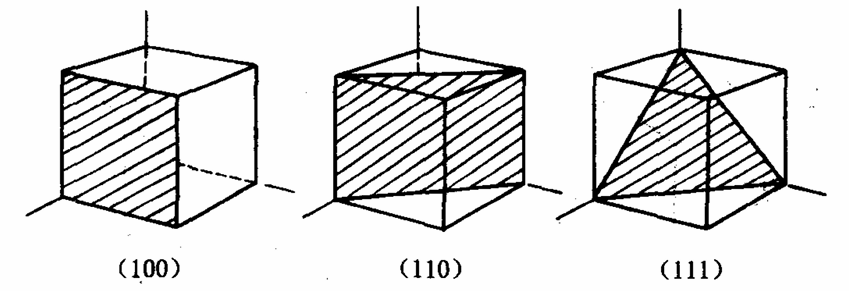
\includegraphics[height=8em, keepaspectratio=true]{pic/1-35}
        \caption{晶面指数}
        \label{fig:1-11}
    \end{figure}

    与等效晶向同理,我们认为具有相同晶体性质的晶面是等效的,即\textbf{等效晶面}\index{等效晶面}。

    例如,立方晶格的表面一共有$(100)$、$(\overline{1}00)$、$(010)$、$(0\overline{1}0)$、$(001)$、$(00\overline{1})$六个晶面,考虑晶格的平移对称性,晶体在这些晶面上的性质是完全相同的。我们用$\{h_1,h_2,h_3\}$来标志一组对称且等效的晶面,即$\{100\}$。

    等效晶面总结如\autoref{tab:1-9}所示:
    \begin{table}[!htbp]
        \centering
        \resizebox{\textwidth}{!}{
        \setlength{\tabcolsep}{1em}
        \begin{tabular}{ccccc}
            \toprule
            &   晶面     & 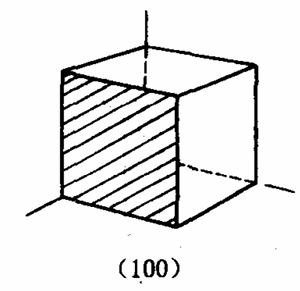
\includegraphics[valign=m, height=4em, keepaspectratio=true]{pic/1-36} & 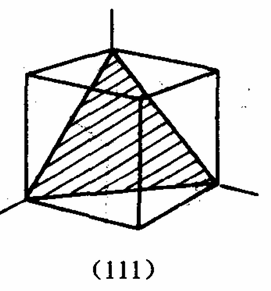
\includegraphics[valign=m, height=4em, keepaspectratio=true]{pic/1-37} & 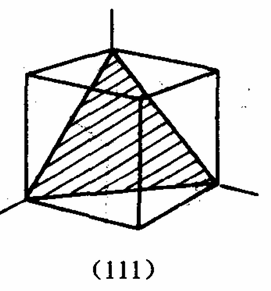
\includegraphics[valign=m, height=4em, keepaspectratio=true]{pic/1-38} \\ \\
            \hline
            \multirow{3}{*}{\textbf{晶向}} & 法线     & 边 & 面对角线 & 体对角线  \\
                                           & 法线数   & 6 & 12 & 8 \\
                                           & 等效晶向 & $<100>$ & $<110>$ & $<111>$ \\
            \hline
            \multirow{3}{*}[-3em]{\textbf{晶面}} & 晶面数   & 6 & 12 & 8 \\
                                           & 等效晶面 & 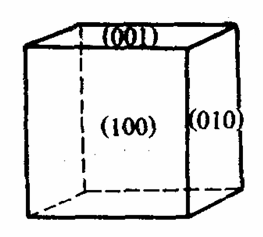
\includegraphics[valign=m, height=4em, keepaspectratio=true]{pic/1-39} & 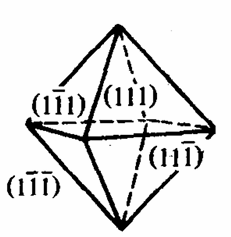
\includegraphics[valign=m, height=4em, keepaspectratio=true]{pic/1-40} & 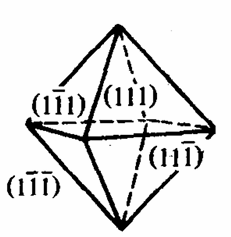
\includegraphics[valign=m, height=4em, keepaspectratio=true]{pic/1-41} \\
                                           & 等效晶面 & $\{100\}$ & $\{110\}$ & $\{111\}$ \\
            \bottomrule
        \end{tabular}
        }
        \caption{等效晶面}
        \label{tab:1-9}
    \end{table}

\subsubsection{密勒指数}
    无论是晶向指数还是晶面指数,都依托于所选取的基矢。
    
    当所选取的晶胞是单胞时,记此时的晶面指数为\textbf{密勒指数}\label{密勒指数},用$\{h, k, l\}$表示;当所选取的晶胞是原胞时,记此时的晶面指数为$\{h_1, h_2, h_3\}$。

    如\nameref{tab:1-7}所述,考虑到:
    \begin{itemize}[itemsep=0pt,parsep=0pt]
        \item 单胞与原胞的基矢在方向、长度上可能不同;
        \item 单胞实际上是扩大了的原胞,从而原胞可以完全反映布拉菲格子的平移对称性,而单胞所反映的对称性是基于平移矢量$\vec{R_l}$的子集,只能沿着结晶轴方向,从而只能局部反映布拉菲格子的平移对称性。
    \end{itemize}
    通过沿坐标轴方向平移单胞,可能无法得到所有的布拉菲格子中的结点,存在遗漏的可能性,进而导致晶面指数中某些晶面的丢失。

    如\autoref{fig:1-12}所示,左侧采用原胞,右侧采用单胞。从而左侧完全无遗地包含所有结点,而右侧的单胞做平移,将沿结晶轴方向平移晶格常数$a$,将无法包含黄色晶面所示的若干结点。右图中黄色晶面,若采用左图的原胞基矢,计算晶面指数为$(101)$,而采用右图的单胞基矢,计算密勒指数为$(100)$,即存在晶面的丢失,这也正是单胞平移时遗漏的结点所构成的晶面。

    \begin{figure}[!htbp]
        \centering    
        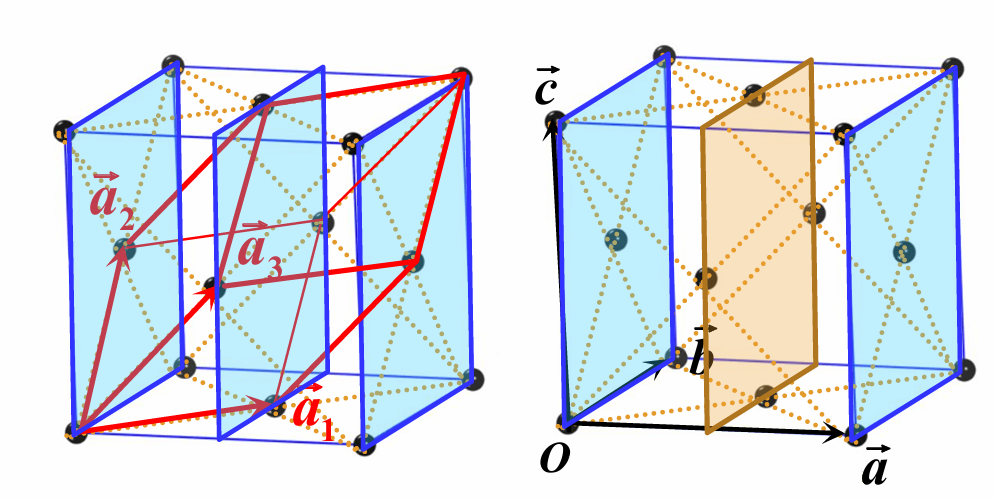
\includegraphics[height=12em, keepaspectratio=true]{pic/1-42}
        \caption{单胞可能导致晶面的丢失}
        \label{fig:1-12}
    \end{figure}

    因此立方单胞的密勒指数可能与其原胞的晶面指数不同。可以证明,立方体结构中,晶面的密勒指数与晶面法线方向的晶向指数完全相同。当密勒指数与晶面指数一致时,可以通过计算晶向指数,快速得到晶面指数,这也是计算晶面指数的另一种方法。
    
    具体来说,\autoref{tab:1-9}中就给出了立方体结构晶格常用晶面的晶面指数,及其法线的晶向指数,二者是完全相同的。


\section{晶体的宏观对称性}

\chapter{倒格子与波矢空间}\label{chap:2}
\section{倒格子}
\section{布里渊区}
\section{X射线衍射}

\chapter{晶格振动}
\section{一维单原子链的振动}
\section{一维双原子链的振动}
\section{三维晶格的振动}

\chapter{能带理论}
\section{自由电子近似}
\section{近自由电子近似}
\section{紧束缚近似}